TODO intro


\subsection{CPUID Instruction}
\label{sec:approach-cpuid}

\mvf{Draft:}

P{\'e}k {\em et al.}~\cite{nether}

Ether alters the output of {\tt CPUID}, flipping the bit for TSC support. Should
be 1 in both VMM and bare metal environment. Can easily be checked, as
Figure~\ref{fig:cpuid-tsc}

If it is a bug in the Ether implementation, best solution is to fix.

Alternatively, if not possible to fix, spoof the value in the same manner as
{\tt PUSHF} and {\tt POPF}. Ether deliberately changes the flag register when
running, as it sets the debug flag to be able to step through the target program
and get a program trace. It hides this from the target by spoofing the values of
instructions used to read and write these flags, as {\tt PUSHF} and {\tt POPF}.
The exact same technique could be used to spoof the TSC-bit when program
executes CPUID.

\begin{figure}[h]
\begin{lstc}
#define CPUID_GETFEATURES 0x00000001
#define CPUID_FEAT_EDX_TSC (1 << 4)
...
__asm__ volatile ("cpuid" :
    "=a" (regs->rax),
    "=b" (regs->rbx),
    "=c" (regs->rcx),
    "=d" (regs->rdx)
    : "a" (CPUID_GETFEATURES), "c" (0));

tsc  = (regs->rdx & CPUID_FEAT_EDX_TSC);

if (!tsc) printf("detected ether!\n");
\end{lstc}
\caption{\label{fig:cpuid-tsc} Code snippet in C showing how to check for TSC
  support through the CPUID instruction.}
\end{figure}

This technique of spoofing the CPUID output suffers from timing attacks, which
will be elaborated in~\nameref{sec:approach-timing}.


\subsection{CPU Errata}
\label{sec:approach-errata}
CPU errata refer to the collection of design defects or errors that may induce the CPU to behave differently from the published specification. Such CPU errata is strongly bound to CPU models and nEther exploits bugs in the Core 2 Duo family, called AH4 Erratum. The AH4 Erratum states that "VERW/VERR/LSL/LAR" instructions may unexpectedly update the Last Exception Record(LER) MSR" and there is no planned fix for it. Concretely, VERW and VERR instructions verify whether the code or data segment specified with the source operand is readable (VERR) or writable (VERW) from the current privilege level. The LAR instruction loads access rights from a segment descriptor into a general purpose register, and the LSL instruction loads the unscrambled segment limit from the segment descriptor into a general-purpose register. This erratum is a design fault so its existence is unintended. Therefore, hardware-assisted-virtualization solutions (e.g., Xen) will not implement this erratum in the virtual CPUs of guests, because there is no need to mimic even unexpected system bugs. As a result, malware can detect hardware-assisted virtualization environment by executing those buggy instructions and checking whether LER MSR is unexpectedly updated or not. In other words, this attack cannot recognize the presence of Ether, but can reveal the hardware-virtualized runtime environment. \\

To thwart this attack completely, we should patch those buggy instructions or use another CPU, but It seems like infeasible and make no sense. So, we propose a practical method to mitigate this attack.

\begin{figure}[!h]
	\centering
	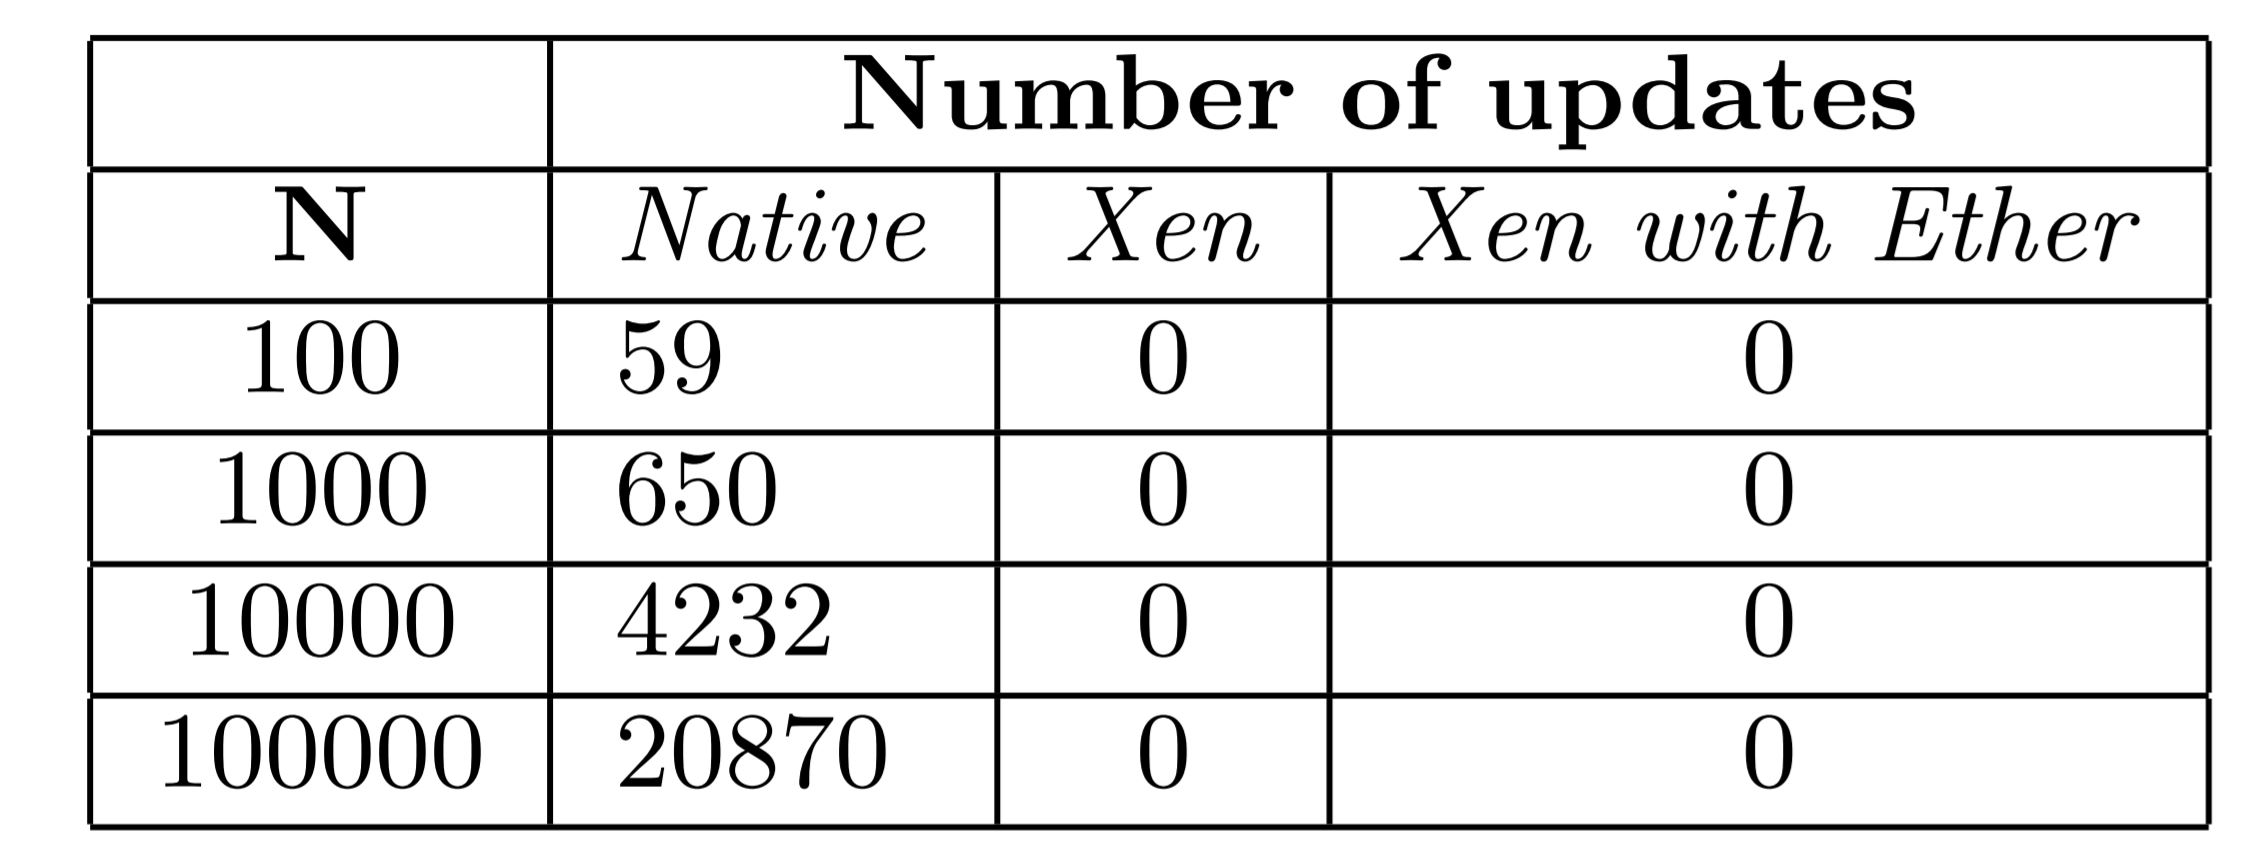
\includegraphics[width=\linewidth]{figure/errata_table.png}
	\caption{The number of LER MSR updates according to the erratum execution}
	\label{fig:errata}
\end{figure}


\subsection{Timing Information}
\label{sec:approach-timing}

todo


%%% Local Variables:
%%% mode: latex
%%% TeX-master: "paper"
%%% End:
